\section{Journey planning}
\label{sec:etas-journey-planning}

So far we have been concerned with the arrival time of a bus at a single stop with no consideration of the passenger's commute as a whole. The simplest journey consists of a single route choice, so the only decision is which trip to catch; a slightly more complex journey may offer two alternative routes (\cref{sec:journey_simple}) which the passenger may choose between. Finally, there may be no single route which goes from the passenger's start location to their destination, in which case a transfer between two (or more) different routes, or \emph{legs}, is necessary (\cref{sec:journey_transfer}).


Since dynamic routing---the selection of candidate trips and \rt{} assessment of which is \emph{optimal}---is in itself a difficult problem to solve \citep{Hame_2013a,Hame_2013b,Zheng_2016}, and there exists implementaions which can take a probabilistic model of arrival time (such as we can obtain by \glspl{cdf}) as input to determine the optimal route (including selecting candidate routes), such as proposed by \citet{Berczi_2017}. Therefore, for this section we only consider choosing between prespecified candidate journey options using the arrival time \glspl{cdf} obtained using our \pf{} model. These are compared to the results one might obtain using the currently deployed schedule-delay method, which can only provide a binary (`Yes' or `No') prediction.


\begin{knitrout}\small
\definecolor{shadecolor}{rgb}{0.969, 0.969, 0.969}\color{fgcolor}\begin{figure}

{\centering 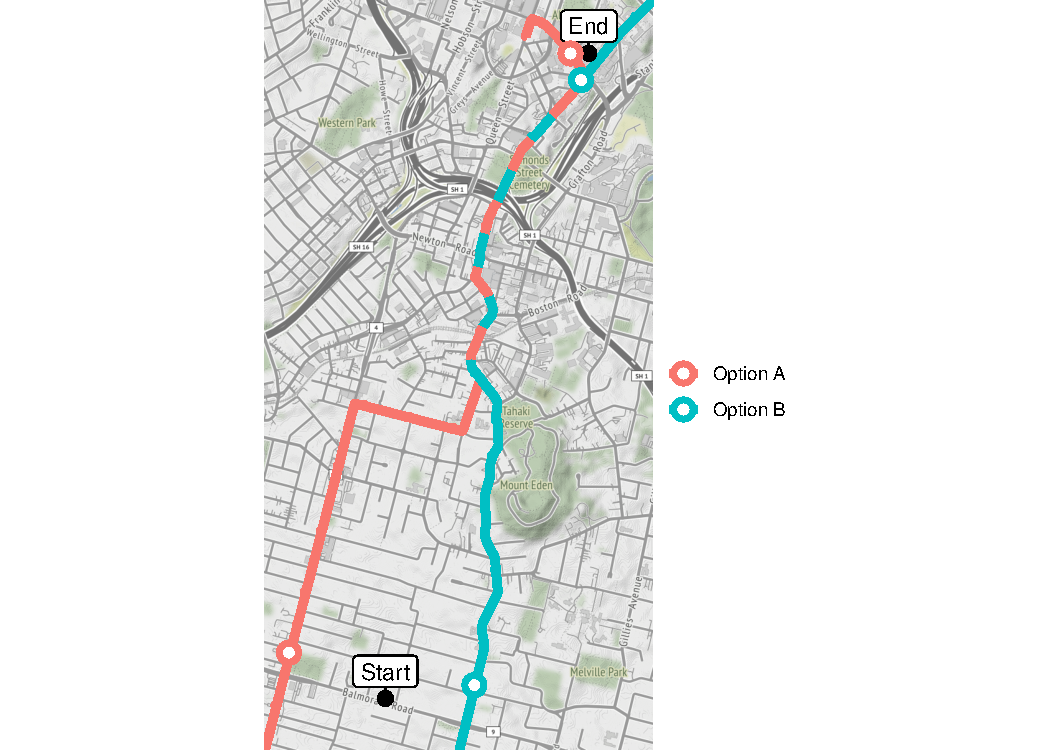
\includegraphics[width=\textwidth]{figure/eta_journey_arrival_prep-1} 

}

\caption[Route options]{Route options}\label{fig:eta_journey_arrival_prep}
\end{figure}


\end{knitrout}

\subsection{Choosing between two alternative routes}
\label{sec:journey_simple}

In this scenario, a passenger lives within walking distance of two major roads, along which various routes travel into the central city, as displayed in \cref{fig:eta_journey_arrival_prep}. The passenger needs to decide which route option to take before leaving home, and let's say they have an appointment in town at 14h00. At 13h20, they consult the real-time app on their phone before deciding whether they will walk to route option A or B. Factors that could influence their decision include:
\begin{itemize}
\item How long will I have to wait until the next bus?
\item What is the probability I will arrive in time for the next bus? And how long until the bus after it?
\item What is the probability that I will arrive at my destination on-time? And how early will I be?
\item How long will I be on the bus?
\end{itemize}
We can answer these questions using the \glspl{cdf} of arrival time at the start and end stops. Walking times at either end of the journey can also be accounted for.


\begin{knitrout}\small
\definecolor{shadecolor}{rgb}{0.969, 0.969, 0.969}\color{fgcolor}\begin{figure}

{\centering 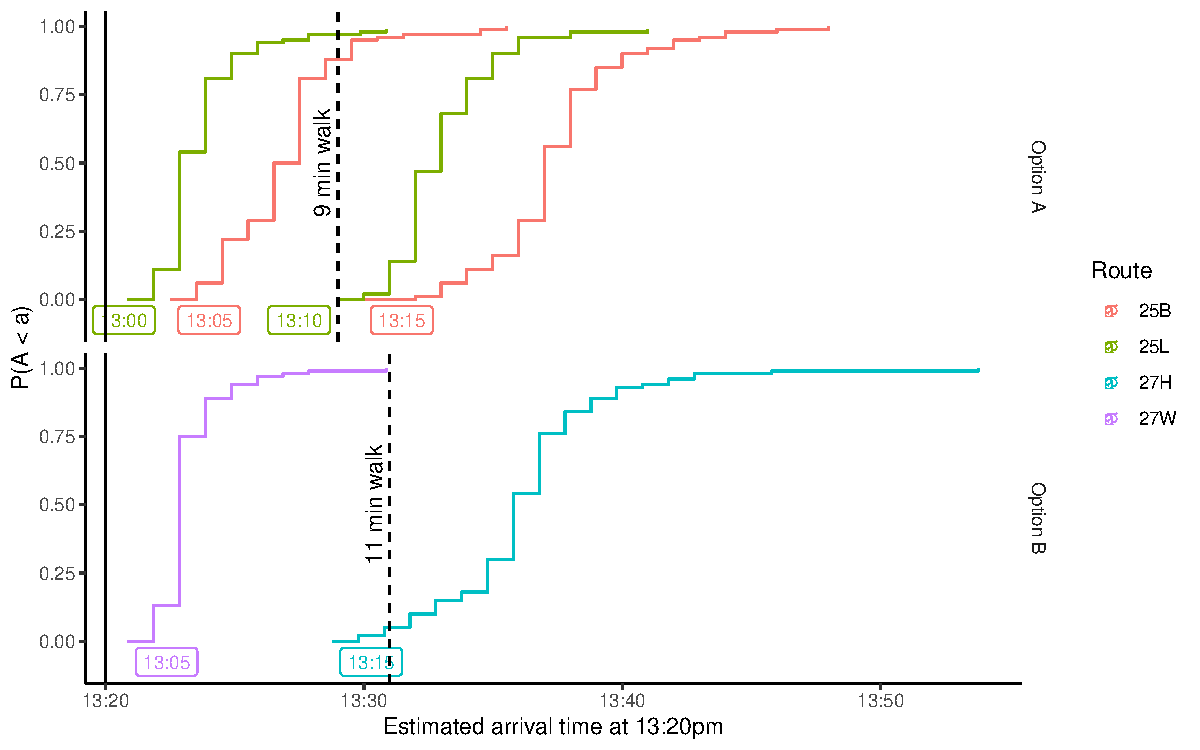
\includegraphics[width=\textwidth]{figure/eta_journey_arrival-1} 

}

\caption[ETA predictions for two route options]{ETA predictions for two route options. The coloured curves represent the CDF of arrival time for individual trips made at 7am. The vertical black lines indicate the estimated walking time (according to Google Maps) from the Start location to each stop.}\label{fig:eta_journey_arrival}
\end{figure}


\end{knitrout}




\Cref{fig:eta_journey_arrival} displays the \glspl{cdf} of all active trips\footnote{Our application currently only estimates arrival times for active trips.} along the two route options at 13h20 when the passenger is about to leave home (solid line), and includes dashed lines representing the passengers arrival time at the stops (accounting for walking time). At the lower end of each \gls{cdf} is a label indicating the trip's start time, which is the simplest method of identifying trips, and the curves are coloured by the route number. For option A, there appears to be a very small chance of catching the 13:05 25B, but a good chance of catching the 13:10 25L, with the additional safety of another 25B not long after. As for option B, there is a slightly smaller chance of catching the 13:15 27H, but if missed it is unclear how long the wait for the next one will be.


\begin{knitrout}\small
\definecolor{shadecolor}{rgb}{0.969, 0.969, 0.969}\color{fgcolor}\begin{figure}

{\centering 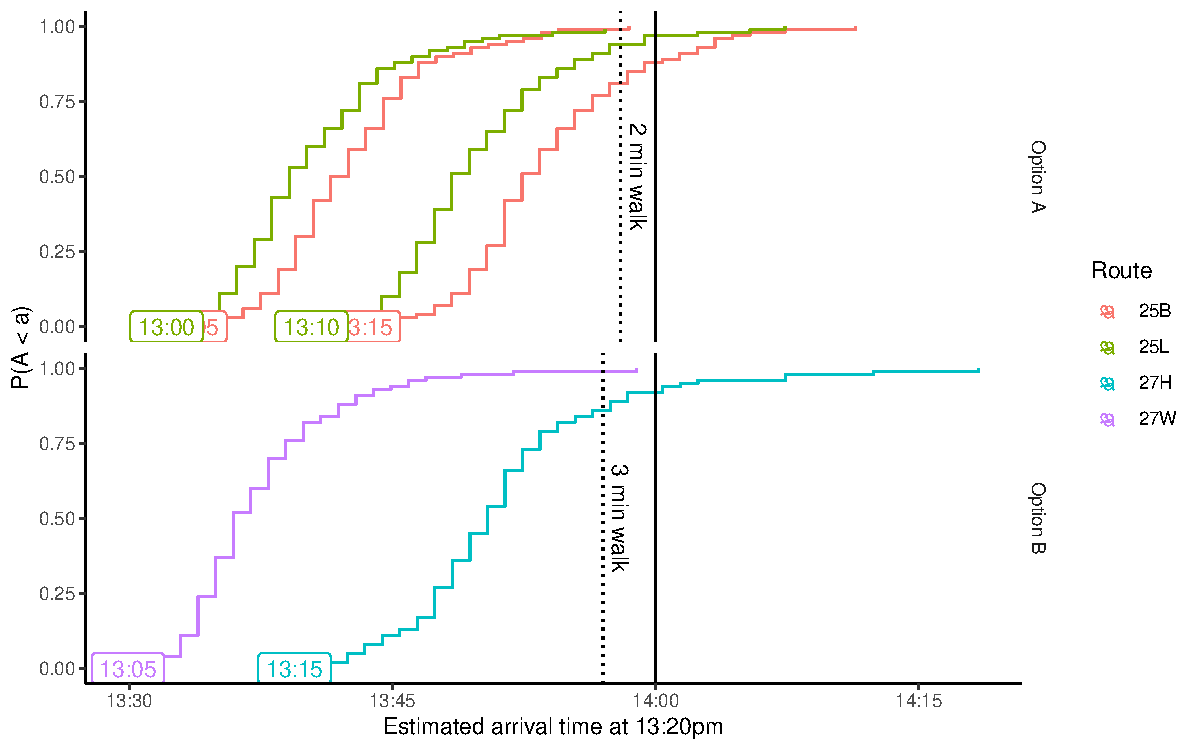
\includegraphics[width=\textwidth]{figure/eta_journey_arriveby-1} 

}

\caption[ETA predictions for two route options]{ETA predictions for two route options. The coloured curves represent the CDF of arrival time for individual trips made at 7am. The vertical black lines indicate the estimated walking time (according to Google Maps) from the Start location to each stop.}\label{fig:eta_journey_arriveby}
\end{figure}


\end{knitrout}

Based on the arrival results alone, it would likely make sense to walk to option A (a shorter walk) which has a decent chance of a short wait time; however, the passenger also need to consider their appointment at 9~am. \Cref{fig:eta_journey_arriveby} provides \glspl{cdf} of each trip's arrival time at the final stop, as well as vertical lines representing the appointment time (solid) and necessary arrival time to account for walking time (dotted). None of the trips show definitive signs of being late, although the passenger would likely hope to catch the 13:10 25L to maximise their chances of arriving on-time, thus confirming the passenger's choice of walking to option A\footnote{At least, that would be my decision.}.


\begin{knitrout}\small
\definecolor{shadecolor}{rgb}{0.969, 0.969, 0.969}\color{fgcolor}\begin{table}

\caption{\label{tab:eta_journey_results}Journey planning.}
\centering
\fontsize{8}{10}\selectfont
\begin{tabular}[t]{lllrrllll}
\toprule
\multicolumn{1}{c}{} & \multicolumn{1}{c}{} & \multicolumn{1}{c}{} & \multicolumn{2}{c}{Particle filter} & \multicolumn{2}{c}{GTFS} & \multicolumn{2}{c}{Outcome} \\
\cmidrule(l{3pt}r{3pt}){4-5} \cmidrule(l{3pt}r{3pt}){6-7} \cmidrule(l{3pt}r{3pt}){8-9}
Option & Route & Trip & $P_\text{catch}$ & $P_\text{arrive}$ & Catch & Arrive & Caught & Arrived\\
\midrule
A & 25L & 13:00 & 0.02 & 0.99 & N & Y & N & Y\\
 & 25B & 13:05 & 0.05 & 0.99 & N & Y & N & Y\\
 & 25L & 13:10 & 0.98 & 0.94 & Y & Y & Y & Y\\
 & 25B & 13:15 & 1.00 & 0.81 & Y & N & Y & Y\\
\midrule
B & 27W & 13:05 & 0.00 & 0.99 & N & Y & N & Y\\
 & 27H & 13:15 & 0.90 & 0.86 & Y & Y & Y & Y\\
\bottomrule
\end{tabular}
\end{table}


\end{knitrout}


The predicted probability of success in each scenario can easily be calculated from the \glspl{cdf}, and are displayed in \cref{tab:eta_journey_results}. Additionally, the binary (`Yes' or `No') predictions according to the schedule-delay method are also displayed for comparison, as well as the eventual outcome (that is, would the passenger have caught the bus and did the bus arrive on time?). All of the predictions based on the \pf{} arrival time \glspl{cdf} are valid: small probabilites had a negative outcome, while large probabilities (>0.8) had a positive one. However, the schedule-delay predictions had one incorrect prediction for the arrival of the 13:15 25B at the destination on time; our method predicted an 81\% chance of success for this route.







\begin{knitrout}\small
\definecolor{shadecolor}{rgb}{0.969, 0.969, 0.969}\color{fgcolor}\begin{figure}

{\centering 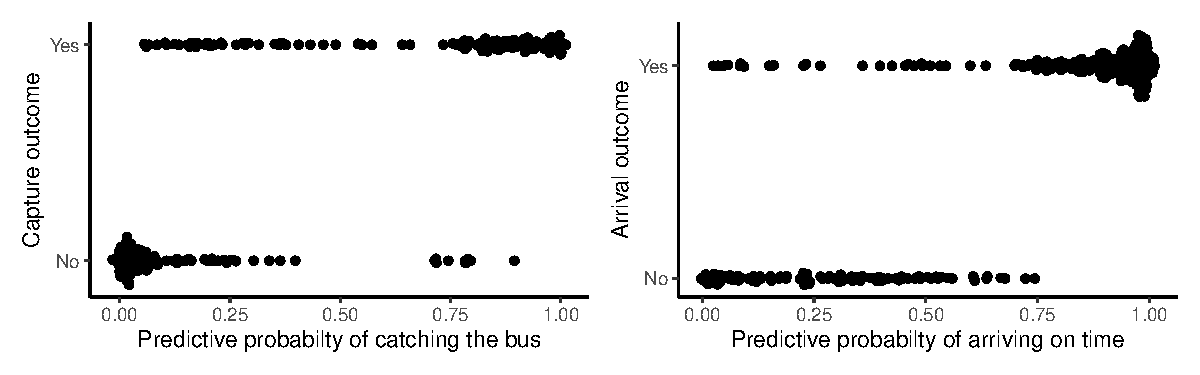
\includegraphics[width=\textwidth]{figure/eta_journey_results_avg-1} 

}

\caption[Results of performing the same journey planning prediction with different starting times (from  9h00 to 15h00), using the same start and end locations]{Results of performing the same journey planning prediction with different starting times (from  9h00 to 15h00), using the same start and end locations. Observations are whether or not the passenger would have arrived at the stop before the bus, jittered to better see each observation. Predictive probabilities of 0 and 1 that were correctly estimated have been removed.}\label{fig:eta_journey_results_avg}
\end{figure}

\begin{table}

\caption{\label{tab:eta_journey_results_avg}GTFS prediction results over all journeys, with the displayed values representing the proportion of outcomes in each cell (rows are conditioned by the GTFS prediction of Yes or No. }
\centering
\fontsize{8}{10}\selectfont
\begin{tabular}[t]{llllll}
\toprule
\multicolumn{1}{c}{} & \multicolumn{5}{c}{Observed outcome} \\
\cmidrule(l{3pt}r{3pt}){2-6}
\multicolumn{1}{c}{ } & \multicolumn{2}{c}{Catch bus} & \multicolumn{1}{c}{} & \multicolumn{2}{c}{Arrive on time} \\
\cmidrule(l{3pt}r{3pt}){2-3} \cmidrule(l{3pt}r{3pt}){5-6}
GTS Prediction & No & Yes &  & No & Yes\\
\midrule
No & 0.98 & 0.02 &  & 0.78 & 0.22\\
Yes & 0.09 & 0.91 &  & 0 & 1\\
\bottomrule
\end{tabular}
\end{table}


\end{knitrout}

The results in \cref{fig:eta_journey_arrival,fig:eta_journey_arriveby} and \cref{tab:eta_journey_results} are based on \emph{one single forecast} made at 13h20. To evaluate the overall performance of our prediction method, we repeated the process described above in 5~minute intervals over the off-peak period from  9h00 to 15h00. For the appointment time, we used 30~minute intervals allowing for 15--45 minutes for the journey: leaving between 9h15 and 9h44 had a targetted arrival time of 8h00; 9h45--10h14 targetted 8h30; and so on. The probabilities of catching the bus and arriving on time were calculated for each case. In \cref{fig:eta_journey_results_avg}, we have graphed the distribution of predicted probabilities for each of the two outcomes, for both catching the bus and arriving on time. Only a small number of missed buses had predictions over 50\%, though a larger number of potential buses had low capture probabilities. As for the arrival outcome, successfully arriving on time was usually predicted well, with a small number of low predictions; however, the maximum probability assigned to a failed on-time arrival was 75\%.



For comparison, \cref{tab:eta_journey_results_avg} presents a two-way contingency table for the binary schedule-delay predictions, with the predicted outcomes in rows. In 91\% of the cases where the bus was predicted to arrive after the passenger was the schedule-delay method correct, and 98\% for when it predicted the passenger would miss the bus. For arrival on time, the bus correctly predicted `Yes' 100\% of the time, but only correctly predicted `No' in 78\% of cases. Overall, the schedule-delay method correctly predicted the bus capture in 94\% of cases, and correctly predicted on-time arrival in 89\% of cases.


In both methods, predicting bus capture is more accurate than predicting on-time arrival, since the forecast length is shorter (10~minutes versus 30~minutes). The schedule-delay predictions give a 1-in-10 chance of missing the bus, while our \pf{} provides a less definite prediction (such as 75\%). This opens up the possiblity for passengers to make more informed decisions based on these probabilites and the importance of their constraints, whereas the schedule-delay method can provide, at best, the predicted arrival time as a singular point estimate with no associated uncertainty.





\subsection{Planning a multi-stage journey}
\label{sec:journey_transfer}

A more complex scenario is one in which the passenger must transfer from one route onto another. Transfer journeys are common for travellers commuting from further afield, where there are often several \emph{feeder routes} which connect at a major hub which usually has more frequent trips to another hub. It may also happen that there simply is no single route between a passengers origin and destination, as is demonstrated in \cref{fig:eta_journey_arrival_prep}. In this scenario, the passenger must first catch a bus along route group A\footnote{We use route groups since there are several different routes which make the same journey, as can be seen with route group B in the south-west of \cref{fig:eta_journey_arrival_prep}.} to the stop marked ``Transfer'', at which point they disembark and wait for the next bus along route group B to get to their final destination (marked ``End'').



\begin{knitrout}\small
\definecolor{shadecolor}{rgb}{0.969, 0.969, 0.969}\color{fgcolor}\begin{figure}

{\centering 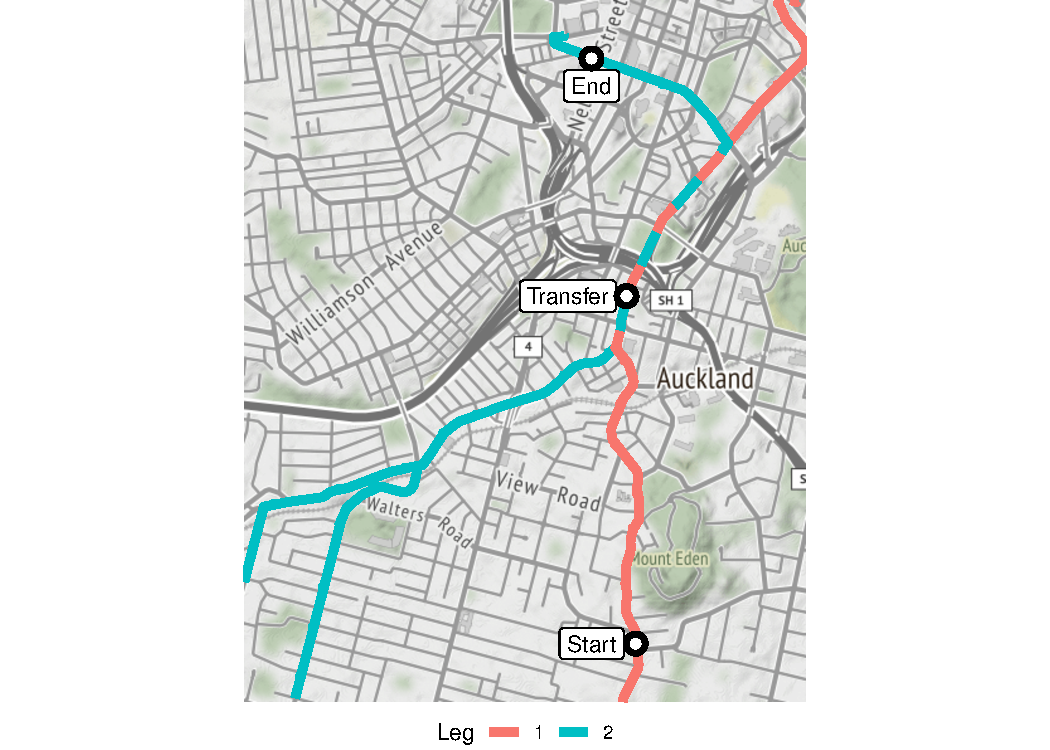
\includegraphics[width=\textwidth]{figure/eta_journey_transfer_prep-1} 

}

\caption[Transfer options]{Transfer options}\label{fig:eta_journey_transfer_prep}
\end{figure}


\end{knitrout}



\begin{knitrout}\small
\definecolor{shadecolor}{rgb}{0.969, 0.969, 0.969}\color{fgcolor}\begin{figure}

{\centering 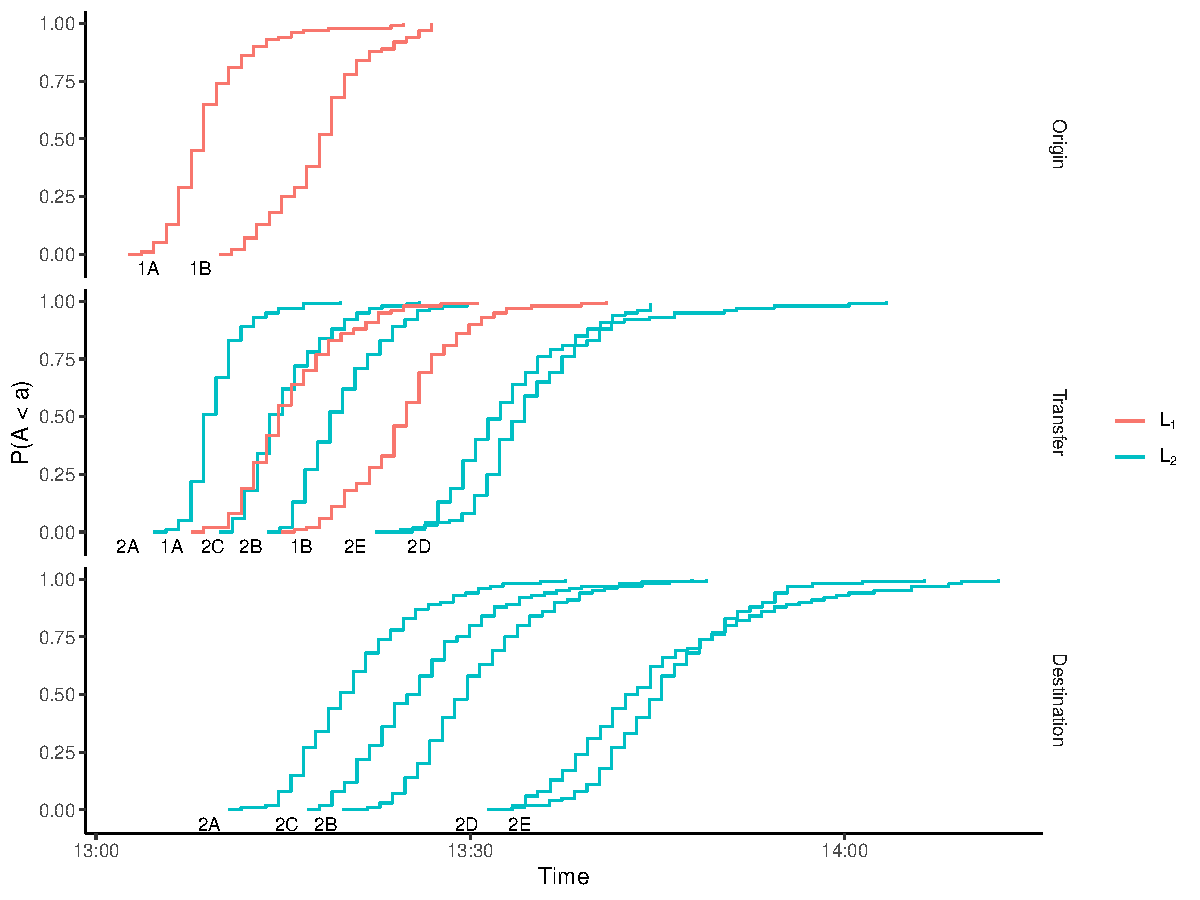
\includegraphics[width=\textwidth]{figure/eta_journey_transfer_graph-1} 

}

\caption[Arrival times]{Arrival times}\label{fig:eta_journey_transfer_graph}
\end{figure}


\end{knitrout}


Similarly to the previous example, we take one single forecast of all trip arrivals at 1~pm to make decisions. Walking time has been removed to simplify the example, but could easily be included if desired. \Cref{fig:eta_journey_transfer_graph} shows, for all active trips at 13h00, their arrival time \glspl{cdf} at the start and transfer stops (for the first leg) and the transfer and end stops (for the second). Additional constraints, such as arrival by a specific time, could of course be added, in this instance we are solely interested in how well a successful transfer can be predicted.


Given \glspl{cdf} for two trips arriving at a stop, the probability that a transfer can successfully be made from A to B can be obtained by the following:
\begin{equation}
\label{eq:eta_total_prob}
\begin{split}
\Pcatch =
\Pr{A < B} &= \sum_{x=1}^{\infty} \Pr{A < B\,|\,B = x}\Pr{B=x} \\
  &= \sum_{x=1}^\infty
    \Pr{A < x} \Pr{B=x} \\
  &= \sum_{x=1}^\infty
    \Pr{A < x} \left[
      \Pr{B < x + 1} - \Pr{B < x}
    \right]
\end{split}
\end{equation}
which we can easily compute given the \glspl{cdf} of the arrival time of each trip obtained from \cref{eq:pf_pdf_arrivaltime}. Table \cref{tab:eta_journey_transfer_res} displays the results, along with the binary predictions using the schedule-delay method along with the observed outcomes. The \pf{} predicts transfer probabilities with reasonable accuracy, with low probabilities resulting in negative outcomes. In contrast, the schedule-delay predicions fail to correctly predict the outcome of a transfer between A1 and B3: it predicts a successful transfer, but infact it is not, while the particle filter predicted a 32\% chance of success. This is where a prediction probability shows its power, in that a passenger could, where applicable, base their decision on how important it is they make the transfer. While this is a fairly non-exciting example (it's a short wait for the next bus), there are other situations where the headway between trips is 30--60~minutes, in which case missing a transfer by a few minutes would be frustrating. However, until our application has been updated to make predictions for upcoming (and not just active) trips, such examples are not yet available.


\begin{knitrout}\small
\definecolor{shadecolor}{rgb}{0.969, 0.969, 0.969}\color{fgcolor}\begin{table}

\caption{\label{tab:eta_journey_transfer_res}Transfer probabilities}
\centering
\fontsize{8}{10}\selectfont
\begin{tabular}[t]{llrll}
\toprule
Leg 1 & Leg 2 & $\mathbb{P}_\text{transfer} & GTFS & Outcome\\
\midrule
1A & 2A & 0.04 & N & N\\
 & 2B & 0.71 & Y & Y\\
 & 2C & 0.32 & Y & N\\
 & 2D & 1.00 & Y & Y\\
 & 2E & 0.99 & Y & Y\\
\midrule
1B & 2A & 0.00 & N & N\\
 & 2B & 0.20 & N & N\\
 & 2C & 0.05 & N & N\\
 & 2D & 0.96 & Y & Y\\
 & 2E & 0.93 & Y & Y\\
\bottomrule
\end{tabular}
\end{table}


\end{knitrout}



\begin{knitrout}\small
\definecolor{shadecolor}{rgb}{0.969, 0.969, 0.969}\color{fgcolor}\begin{figure}

{\centering 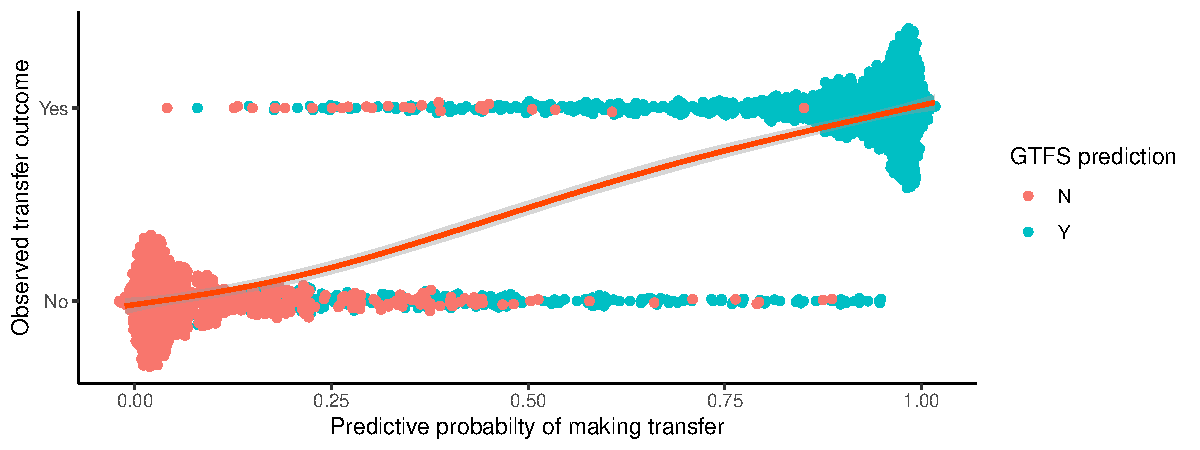
\includegraphics[width=.5\textwidth]{figure/eta_journey_transfer_many-1} 

}

\caption[Results of performing the same transfer journey planning prediction with different starting times (from  9h00 to 15h00)]{Results of performing the same transfer journey planning prediction with different starting times (from  9h00 to 15h00). Observations are whether or not the first bus would arrive at the transfer stop before the second bus, jittered to better see each observation. Additionally, predictive probabilities of 0 and 1 have been removed since, after checking, none or these were invalid and only served to distort the figure.}\label{fig:eta_journey_transfer_many}
\end{figure}

\begin{table}

\caption{\label{tab:eta_journey_transfer_many}Results of running the transfer prediction problem over the course of the day. Rows represent the predicted outcome (No, the transfer will be made, or Yes, it will) and the numbers represent the proportion of predictions with each observed outcome. The GTFS rule is binary, while the particle filter results are based on transfer probability of at least 0.5, 0.8, or 0.95 (as indicated).}
\centering
\fontsize{8}{10}\selectfont
\begin{tabular}[t]{llllllllllll}
\toprule
\multicolumn{1}{c}{} & \multicolumn{11}{c}{Outcome} \\
\cmidrule(l{3pt}r{3pt}){2-12}
\multicolumn{1}{c}{} & \multicolumn{2}{c}{GTFS} & \multicolumn{1}{c}{} & \multicolumn{2}{c}{PF (P > 0.5)} & \multicolumn{1}{c}{} & \multicolumn{2}{c}{PF (P > 0.8)} & \multicolumn{1}{c}{} & \multicolumn{2}{c}{PF (P > 0.95)} \\
\cmidrule(l{3pt}r{3pt}){2-3} \cmidrule(l{3pt}r{3pt}){5-6} \cmidrule(l{3pt}r{3pt}){8-9} \cmidrule(l{3pt}r{3pt}){11-12}
Prediction & No & Yes &  & No & Yes &  & No & Yes &  & No & Yes\\
\midrule
No & 0.97 & 0.03 &  & 0.94 & 0.06 &  & 0.85 & 0.15 &  & 0.7 & 0.3\\
Yes & 0.1 & 0.9 &  & 0.07 & 0.93 &  & 0.03 & 0.97 &  & 0 & 1\\
\bottomrule
\end{tabular}
\end{table}


\end{knitrout}


As before, we proceed to repeat the procedure for multiple times (this time between  9h00 and 15h00), and compute the probabilities of available transfers and whether or not they connected. \Cref{fig:eta_journey_transfer_many} shows the predicted transfer probabilities grouped by outcome, and coloured by the schedule-delay prediction. This is complimented with contingency \cref{tab:eta_journey_transfer_many} for the schedule-delay method and our own, respectively. For the schedule-delay method, in 10\% of cases a predicted successfull connection failed and showed a 3\%, versus only 7\% using the \pf{} with a decision rule of $\Pcatch > 0.5$. The false negative rate was similar for both methods, although slightly higher for our own (6\% versus 3\% for schedule-delay). However, depending on the passenger's requirements, it is possible to reduce the false positive rate under the \pf{} by increasing the threshold. \Cref{tab:eta_journey_transfer_many} also shows the results using 0.8 and 0.95 as the decision rule, which result in a 3\% and 0\% false positive rate, respectively, though these result in quite a significant increase in the false negative rate. Again, by providing probabilities the passenger has the option to decide what level of risk they are willing to take.


In this section we have seen that having access to the full distribution of arrival times enables calculation of event probabilities as opposed to binary outcome predictions. This allows for more sophisticated decision making by travellers depending on their own needs, or by journey planning software. A further advantage of using the \pf{} to estimate the \glspl{cdf} is  that any improvements to the vehicle or network models will automatically be integrated into the arrival prediction component, allowing for further improvments.
